%!TEX root = ../dissertation.tex

\chapter{Evaluation}
\label{chapter:evaluation}
The goal of our work was to bring \gls{gd} to the web browser so it can be used anywhere easily.
In this chapter, we assess how our solution accomplishes this goal.
We start by looking at some examples that were implemented in the environment in Section~\ref{sec:eval:gd:capable}.
Afterwards, we measure the environment's performance and compare it to other environments in Section~\ref{sec:eval:performance}.


\section{GD capability / Usage examples}
\label{sec:eval:gd:capable}
A programming environment needs to allow for the creation of a wide variety of programs.
Now comes the time to test the environment's ability to be used for \gls{gd}, more specifically to produce diverse 3D models.
To show this variety, we will present several examples that make use of some of the primitives that were implemented in the prototype and also some programming techniques that they use.

%(illustrate main results of the implementation?)\\
%(show that environment is able to produce GD models?)\\
%(show techniques that can be used in the environment?)


\subsection{Example: Atomium}
The Atomium in Brussels was built between 1956 and 1958 for Expo 58.
It consists of nine metallic spheres connected by sixteen tubes to form its shape, mimicking the arrangement of an iron crystal structure.

To create it in the environment, we can start by deciding which primitives to use for the elements of the Atomium, that is the metallic spheres and the tubes.
The spheres can be created using the {\tt sphere} primitive.

\begin{minted}{js}
function atomiumSpheres(cs, r) {
  return map(c => sphere.byCenterRadius(c, r), cs);
}
\end{minted}

The tubes can be created using the {\tt cylinder} primitive.
They are placed at the edges of the cube defined by the outside spheres and also at the lines connecting them to the inside sphere.
Sequence generation and manipulation functions -- like {\tt zip}, {\tt rotateLeft}, {\tt repeatTimes}, and {\tt concat} -- are used to create all cylinder center pairs.

\begin{minted}{js}
function atomiumTube(p1, p2, r) {
  return cylinder.byCentersRadius([p1, p2], r);
}

function atomiumTubes(c0, upCs, downCs, r) {
  return [
    map(([p1,p2]) => atomiumTube(p1, p2, r),
      zip(upCs, rotateLeft(upCs, 1))),
    map(([p1,p2]) => atomiumTube(p1, p2, r),
      zip(downCs, rotateLeft(downCs, 1))),
    map(([p1,p2]) => atomiumTube(p1, p2, r),
      zip(upCs, downCs)),
    map(([p1,p2]) => atomiumTube(p1, p2, r),
      zip(repeatTimes(c0, 8), concat(upCs, downCs)))
  ];
}
\end{minted}

Now, the coordinates of each sphere center must be defined and sent to {\tt atomiumSpheres} and {\tt atomiumTubes}.

\begin{minted}{js}
function atomiumFrame(sphereR, frameW, tubeR) {
  let c0 = xyz(0,0,0),
    c1 = xyz(-frameW, -frameW, +frameW),
    c2 = xyz(+frameW, -frameW, +frameW),
    c3 = xyz(+frameW, +frameW, +frameW),
    c4 = xyz(-frameW, +frameW, +frameW),
    c5 = xyz(-frameW, -frameW, -frameW),
    c6 = xyz(+frameW, -frameW, -frameW),
    c7 = xyz(+frameW, +frameW, -frameW),
    c8 = xyz(-frameW, +frameW, -frameW);
  return [
    atomiumSpheres([c0,c1,c2,c3,c4,c5,c6,c7,c8], sphereR),
    atomiumTubes(c0, [c1,c2,c3,c4], [c5,c6,c7,c8], tubeR)
  ];
}
\end{minted}

After creating the structure, we rotate it aligning its $z$ axis with an axis passing through $(0,0,0)$ and $(1,1,1)$.
Figure~\ref{fig:ex:atomium} shows the resulting model.

\begin{minted}{js}
function atomium(sphereR, frameW, tubeR) {
  return rotate(atomiumFrame(sphereR, frameW, tubeR))
    .aligningAxes(axis.z, axis.xyz);
}
\end{minted}

\begin{figure}
  \centering
  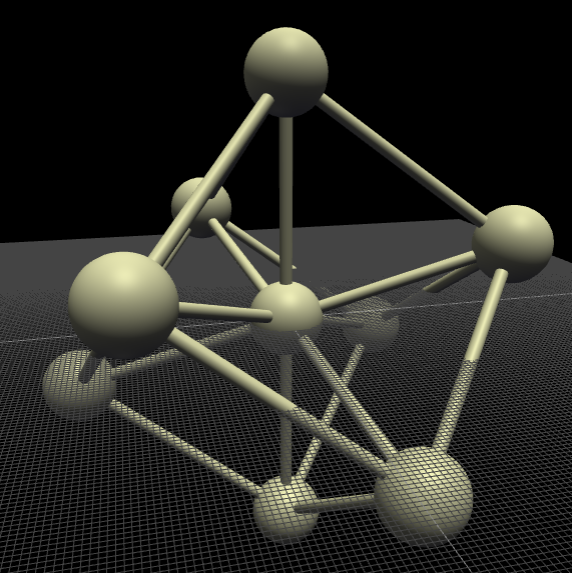
\includegraphics[width=0.5\linewidth]{./images/detail_examples/atomium_2_crop}
  \caption{Atomium}
  \label{fig:ex:atomium}
\end{figure}


\subsection{Example: Trusses}
Trusses are a common element in architecture that can adapt to different surfaces while maintaining strong structural properties.
Trusses often consist of straight members connected together at their extremities, or joints.
They can be planar, meaning that their members all lie on the same plane, or spatial, where members are distributed in three dimensional space.
Spatial trusses can be represented by the mesh formed by their members.
The following program implements spatial trusses with the same topology of a planar space frame:

\begin{minted}{js}
function trussKnots(pts, radius) {
  return map((pt) => sphere.byCenterRadius(pt, radius), pts);
}

function trussBars(ps, qs, radius) {
  return map(([p, q]) => cylinder.byCentersRadius([p, q], radius), zip(ps, qs));
}

function spatialTruss(curves, knotRadius, barRadius) {
  let as = curves[0];
  let bs = curves[1];
  let cs = curves[2];
  return [
    trussKnots(as, knotRadius),
    trussKnots(bs, knotRadius),
    trussBars(as, cs, barRadius),
    trussBars(bs, dropRight(as, 1), barRadius),
    trussBars(bs, dropRight(cs, 1), barRadius),
    trussBars(bs, drop(as, 1), barRadius),
    trussBars(bs, drop(cs, 1), barRadius),
    trussBars(drop(as, 1), dropRight(as, 1), barRadius),
    trussBars(drop(bs, 1), dropRight(bs, 1), barRadius),
    curves.length === 3 ?
      [
        trussKnots(cs, knotRadius),
        trussBars(drop(cs, 1), dropRight(cs, 1), barRadius)
      ]
      : [
        trussBars(bs, curves[3], barRadius),
        spatialTruss(drop(curves, 2), knotRadius, barRadius)
      ]
  ];
}
\end{minted}

The {\tt spatialTruss} function creates a space frame for any set of joint coordinates.
Like so, if we wanted to produce a truss following an arc, we could define it with the following functions:

\begin{minted}{js}
function arcCs(p, r, phi, psi0, psi1, n) {
  return map(psi => add(p, spherical(r, phi, psi)),
    intervalDivision(psi0, psi1, n));
}

function arcTrussCs(p, apexR, baseR, phi, psi0, psi1, e, n) {
  let dpsi = (psi1 - psi0)/n;
  return [
    arcCs(add(p, polar(e/2, phi + Math.PI/2)),
      apexR, phi, psi0, psi1, n),//base arc
    arcCs(p, baseR, phi,
      psi0 + dpsi/2, psi1 - dpsi/2, n-1),//apex arc
    arcCs(add(p, polar(e/2, phi - Math.PI/2)),
      apexR, phi, psi0, psi1, n)//base arc
  ];
}

function arcTruss(p, apexR, baseR, phi, psi0, psi1, e, n) {
  return spatialTruss(
    arcTrussCs(p, apexR, baseR, phi, psi0, psi1, e, n),
    0.3, 0.1);
}
\end{minted}

The {\tt arcCs} function creates a given number of points in an arc.
Function {\tt arcTrussCs} then uses this function to the three arcs that include all the coordinates of joints of the truss.
It is then used in {\tt arcTruss} in conjuntion with {\tt spatialTruss} to actually create the space frame (Figure~\ref{fig:arc:truss}).

\begin{figure}
  \centering
  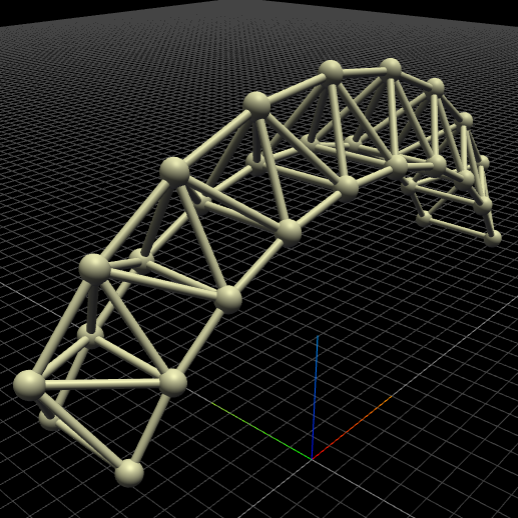
\includegraphics[width=0.5\textwidth]{./images/detail_examples/arc_truss_crop}
  \caption{An arc-shaped truss.}
  \label{fig:arc:truss}
\end{figure}

It is common that planar space frames are required to follow a surface.
Unfortunately, {\tt spatialTruss} requires not only points that lie on the surface but also points that are either below or above it to be able to create the trusses's quadrangular pyramids.
{\tt insertPyramidApexCurves} is an helper function that creates a set of joint coordinates ready for {\tt spatialTruss} from a grid of points by adding pyramid apexes for each quad defined by by the grid.
{\tt spatialTrussInsertApex} combines {\tt insertPyramidApexCurves} and {\tt spatialTruss} into one easy to use function.

\begin{minted}{js}
function insertPyramidApexCurves(curves) {
  let css1 = curves,
    css2 = drop(curves, 1);
  let apexess = map(
    ([cs1, cs2]) => insertPyramidApex2Curves(cs1, cs2),
    zip(css1, css2));
  return interleave(css1, apexess);
}

function spatialTrussInsertApex(cs) {
  let c1 = (cs[0])[0];
  let c2 = (cs[1])[0];
  let c4 = (cs[0])[1];
  let d = Math.min(distance(c1, c2), distance(c1, c4));
  let knotRadius = d/5;
  let barRadius = d/15;
  return spatialTruss(
    insertPyramidApexCurves(cs), knotRadius, barRadius);
}
\end{minted}

With this function, it is possible to create trusses on any surface.
For example, on a wavy surface, as seen in Figure~\ref{fig:truss:wavy}, or on a surface following the Moebius band, as seen in Figure~\ref{fig:truss:moebius}.
%{\bf (drawing heavily from José Lopes' thesis)}\\

\begin{figure}
\begin{minipage}{0.5\textwidth}
\begin{minted}{js}
function wavyCs(p, baseR, l, phi,
  psi0, psi1, psiN,
  alpha0, alpha1, alphaN, rAmpl) {
  return map(
    ([i, alpha]) => arcCs(
      add(p, polar(i*l, phi + Math.PI/2)),
      baseR + rAmpl*Math.sin(alpha), phi,
      psi0, psi1, psiN
    ),
    zip(count(alphaN),
      intervalDivision(
        alpha0, alpha1, alphaN))
  );
}

function wavyTruss(p, baseR, l, phi,
  psi0, psi1, psiN,
  alpha0, alpha1, alphaN, rAmpl) {
  return spatialTrussInsertApex(
    wavyCs(p, baseR, l, phi,
      psi0, psi1, psiN,
      alpha0, alpha1, alphaN, rAmpl));
}
\end{minted}
\end{minipage}%
\begin{minipage}{0.5\textwidth}
  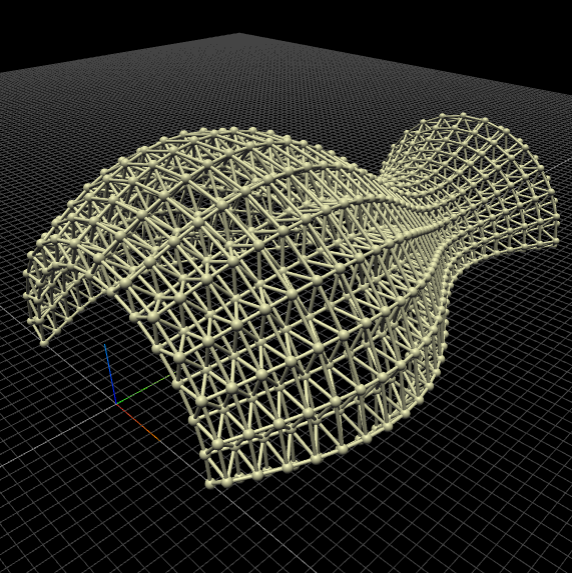
\includegraphics[width=1.0\textwidth]{./images/detail_examples/wavy_truss_crop}
\end{minipage}
\caption{A wavy truss.}
\label{fig:truss:wavy}
\end{figure}

\begin{figure}
\begin{minipage}{0.5\textwidth}
\begin{minted}{js}
function moebiusCs(r, u1, u2, m,
  v1, v2, n) {
  return enumerateMN(function(u, v) {
    return cylindrical(
      r*(1 + (v*Math.cos(u/2))),//radius
      u,//angle
      r*v*Math.sin(u/2));//z
  }, u1, u2, m, v1, v2, n);
}

function moebiusTruss(r, u1, u2, m,
  v1, v2, n) {
  return spatialTrussInsertApex(
    moebiusCs(r, u1, u2, m, v1, v2, n));
}
\end{minted}
\end{minipage}%
\begin{minipage}{0.5\textwidth}
  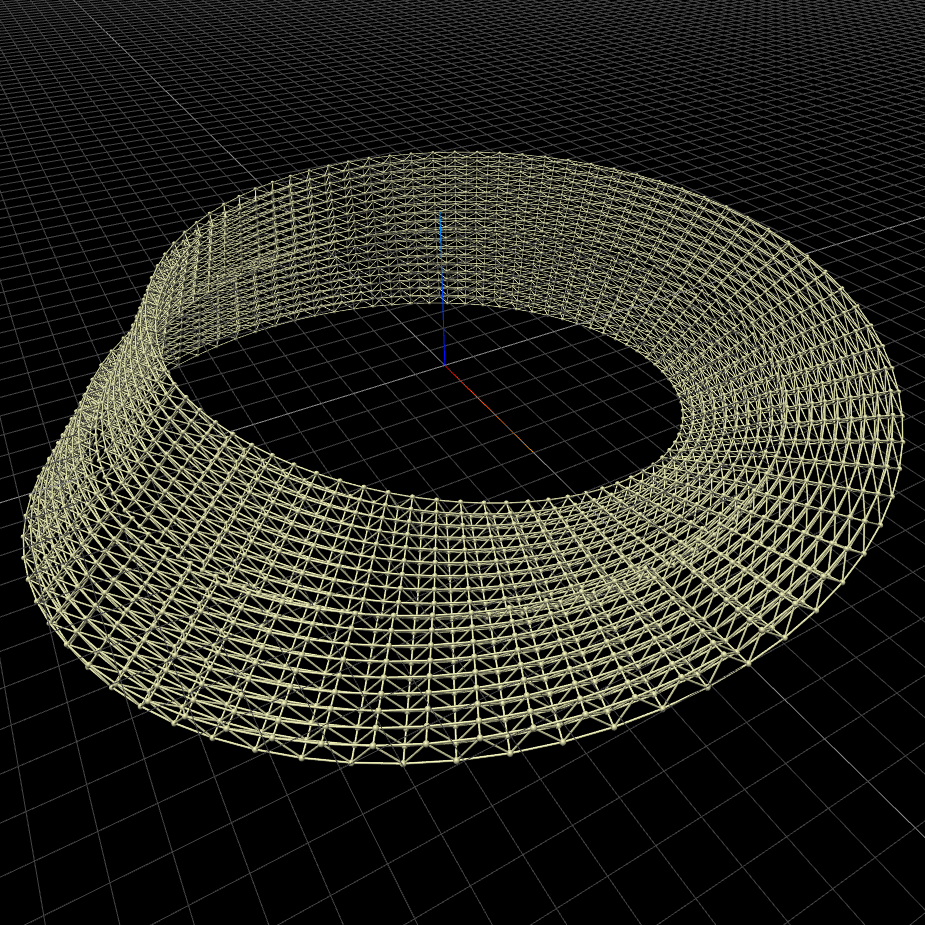
\includegraphics[width=1.0\textwidth]{./images/detail_examples/moebius_truss_crop}
\end{minipage}
\caption{A truss on the moebius band.}
\label{fig:truss:moebius}
\end{figure}


\subsection{Example: Randomness}
Computer programs allow highly repetitive designs to be generated quickly, however, architects may want to introduce some variation to make designs look more natural.
They can do this by introducing randomness into parts of their designs.
The environment supports this by providing functions that generate random numbers.

Randomness can be used to randomize the control-flow of a program or other discrete aspects of the program.
Suppose that we want to create a simplistic city where approximately one third of buildings are cylindrical and two thirds are cubic.
Consider the program:

\noindent
\begin{minipage}{1.0\textwidth}
\begin{minipage}{0.5\textwidth}
\begin{minted}{js}
function coordinateGrid(p, uu, vv, m, n) {
  return map(
    ([u, v]) => add(p,
      add(scale(uu, u), scale(vv, v))),
    cartesianProduct(count(m), count(n))
  );
}

function building(p) {
  return random.real(3) < 1
    ? cylinder.byCentersRadius(
      [p, add(p, z(75))], 10)
    : box.byBottomWidthHeightZ(
      p, [20, 20], 60);
}

function city(p) {
  return map(building,
    coordinateGrid(p, x(25), y(25),
      10, 10));
}
\end{minted}
\end{minipage}%
\begin{minipage}{0.5\textwidth}
  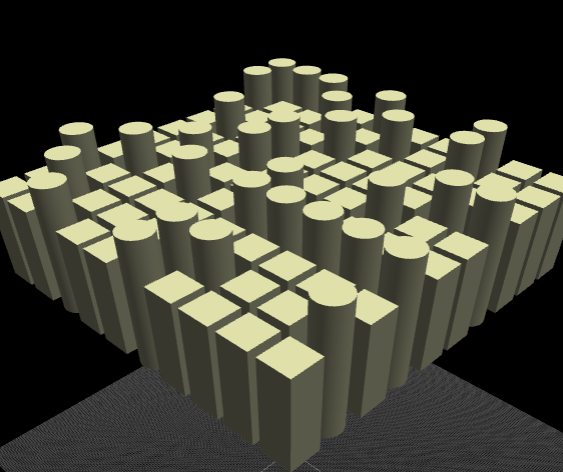
\includegraphics[width=1.0\textwidth]{./images/detail_examples/box_cyl_city_crop}
\end{minipage}
\end{minipage}

The function {\tt building} uses {\tt random.real} to decide whether to create a cylinder or a box.
Calling {\tt city} with a point creates a grid of boxes and cylinders where approximately one third are cylinders, as seen in next. %Figure~\ref{fig:box:cyl:city}.

%\begin{figure}
%  \centering
%  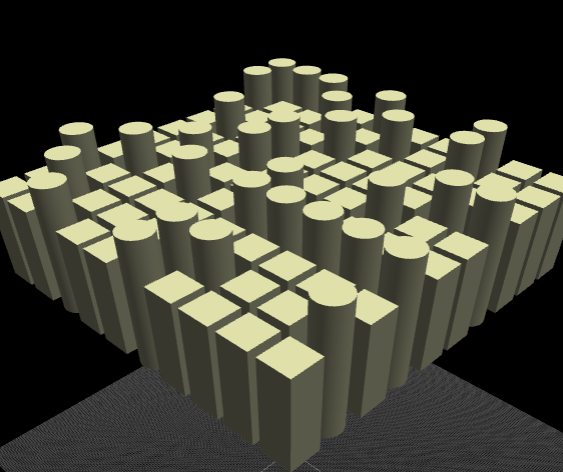
\includegraphics[width=0.5\textwidth]{./images/detail_examples/box_cyl_city_crop}
%  \caption{City of cylinders and boxes.}
%  \label{fig:box:cyl:city}
%\end{figure}

Random numbers can also be used to control continuous quantities like heights or distances.
For example, we can modify function {\tt building} to also pick a random height for the buildings it produces.

\noindent
\begin{minipage}{1.0\textwidth}
\begin{minipage}{0.5\linewidth}
\begin{minted}{js}
function building(p) {
  return random.real(3) < 1
    ? cylinder.byCentersRadius(
      [p, add(p,
        z(random.real.inRange(10, 75)))],
      10)
    : box.byBottomWidthHeightZ(p, [20, 20],
      random.real.inRange(5, 60));
}
\end{minted}
\end{minipage}%
\begin{minipage}{0.5\linewidth}
  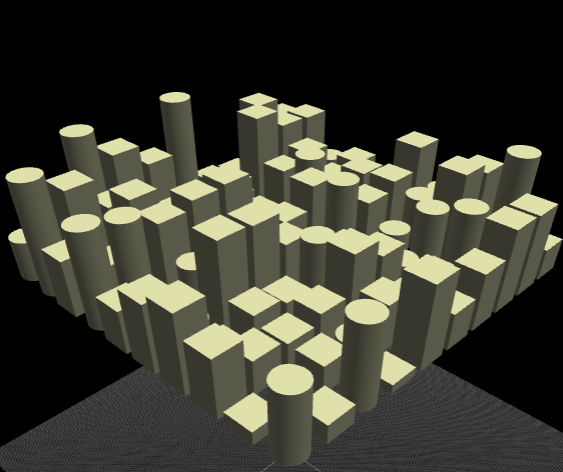
\includegraphics[width=1.0\linewidth]{./images/detail_examples/box_cyl_city_random_crop}
\end{minipage}
\end{minipage}

The examples from Figure~\ref{fig:ex:nolan}, \ref{fig:ex:ines:wall} and \ref{fig:ex:sheung:wan} also make use of random numbers.
The first example uses them to vary the rotation of the square elements of the facade.
The second uses them to decide which areas should have more or less holes and to determine the displacement of bricks from the face of the wall.
Lastly, the third uses random numbers to determine thicknesses of blocks, to determine where to subdivide them, to decide whether to further subdivide or not, and to decide which blocks from the smooth part (the lower part) should look like the ones from the rough part (the upper part).

\begin{figure}
  \centering
  \begin{subfigure}[b]{0.3\linewidth}
    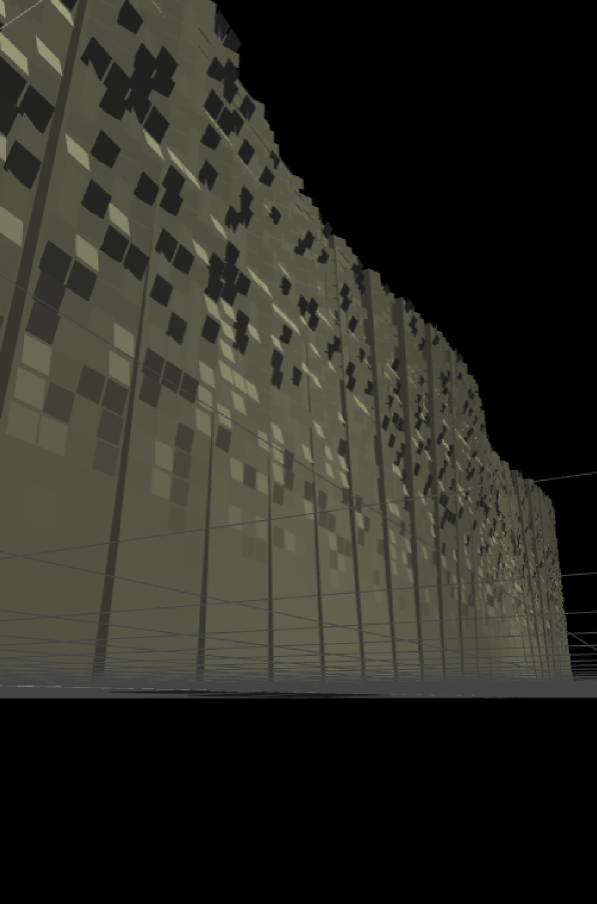
\includegraphics[width=1.0\linewidth]{./images/all_examples/nolan_facade_crop}
    \caption{Nolan Facade}
    \label{fig:ex:nolan}
  \end{subfigure}
  \begin{subfigure}[b]{0.3\linewidth}
    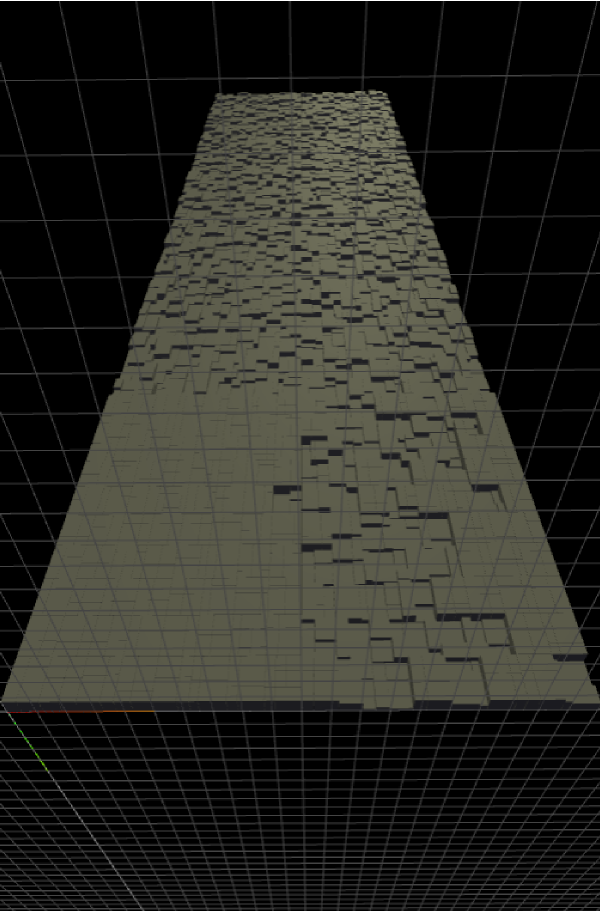
\includegraphics[width=1.0\linewidth]{./images/all_examples/sheung_wan_hotel_crop}
    \caption{Sheung-Wan Hotel}
    \label{fig:ex:sheung:wan}
  \end{subfigure}
  \begin{subfigure}[b]{0.3\linewidth}
    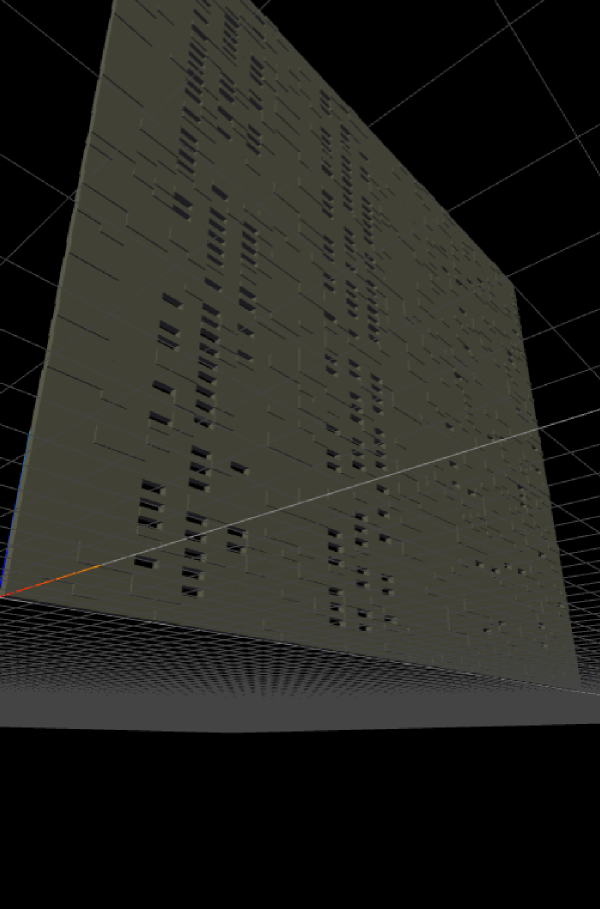
\includegraphics[width=1.0\linewidth]{./images/all_examples/ines_wall_crop}
    \caption{Ines Wall}
    \label{fig:ex:ines:wall}
  \end{subfigure}
  \caption{Results of programs using randomness.}
  \label{fig:rand:progs}
\end{figure}


\subsection{Example: Higher-order Functions}
Higher-order functions are functions that receive functions as parameters and/or return functions as their result.
One benefit that comes from higher-order functions is allowing their behavior to change without requiring them to be modified.

Coming back to the example of creating a simplistic city.
The implementation that was presented earlier was limited in terms of the creation of buildings.
It requires the {\tt building} function to be modified in order to allow the city to have different kinds of buildings.
It would be preferable to turn {\tt city} into an higher-order function receiving the functions responsible for creating the buildings.
The modified function is the following:

\begin{minted}{js}
function city(p, buildingFns) {
  return map(pt =>
    buildingFns[random.integer(buildingFns.length - 1)](pt),
    coordinateGrid(p, x(25), y(25), 10, 10));
}
\end{minted}

With this modification, it becomes possible to creating variations of the city by simply choosing a different set of buildings.
Like so, we can extract the two buildings from {\tt building} into separate functions.
In addition, we can also implement other types of buildings, like the one from {\tt coneBuilding}.

\begin{minted}{js}
function cylBuilding(p) {
  return cylinder.byCentersRadius(
    [p, add(p, z(random.real.inRange(10, 75)))],
    10);
}

function boxBuilding(p) {
  return box.byBottomWidthHeightZ(p, [20, 20],
    random.real.inRange(5, 60));
}

function coneBuilding(p) {
  return coneFrustum.byBottomTopRadiusesHeight(
    p, 10, random.real.inRange(0, 8),
    random.real.inRange(5, 60)
  );
}
\end{minted}

Now we can call {\tt city} with these buildings, as seen in Figure~\ref{fig:cyl:box:cone:city}.

\begin{figure}
\begin{minipage}{0.5\textwidth}
\begin{minted}{js}
  city(xyz(0, 0, 0),
    [cylBuilding, boxBuilding, coneBuilding]);
\end{minted}
\end{minipage}%
\begin{minipage}{0.5\textwidth}
  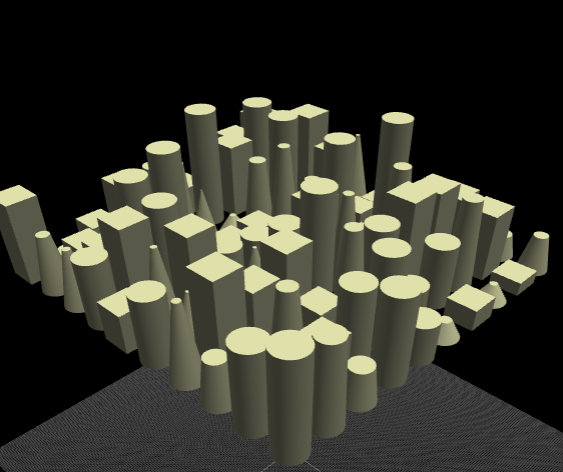
\includegraphics[width=1.0\textwidth]{./images/detail_examples/box_cyl_city_higher_crop}
\end{minipage}
\caption{Making a city of boxes, cylinders and cone frustums.}
\label{fig:cyl:box:cone:city}
\end{figure}


\subsection{Completeness}
Apart from the previous examples, some additional programs made using the environment.
Figure~\ref{fig:all:examples} shows their results.
As shown, the environment can produce interesting results with varying degrees of complexity.
The range of results is still limited by the primitives currently implemented.
For example, none of these programs make use of \gls{csg} operations like union, intersection and difference as they are not implemented.
Nevertheless, it is possible to add support for them since there are already JavaScript implementations of \gls{csg}, like the case of OpenJSCAD's.
The goal of the prototype is only to assess that today's web browsers are able to support a \gls{gd} programming environment.
Like so, it does not need to have all operations that an architect might need.
That would also be unrealistic given the limited time frame of a master's thesis.


\begin{figure}
  \centering
  \begin{subfigure}[b]{0.3\linewidth}
    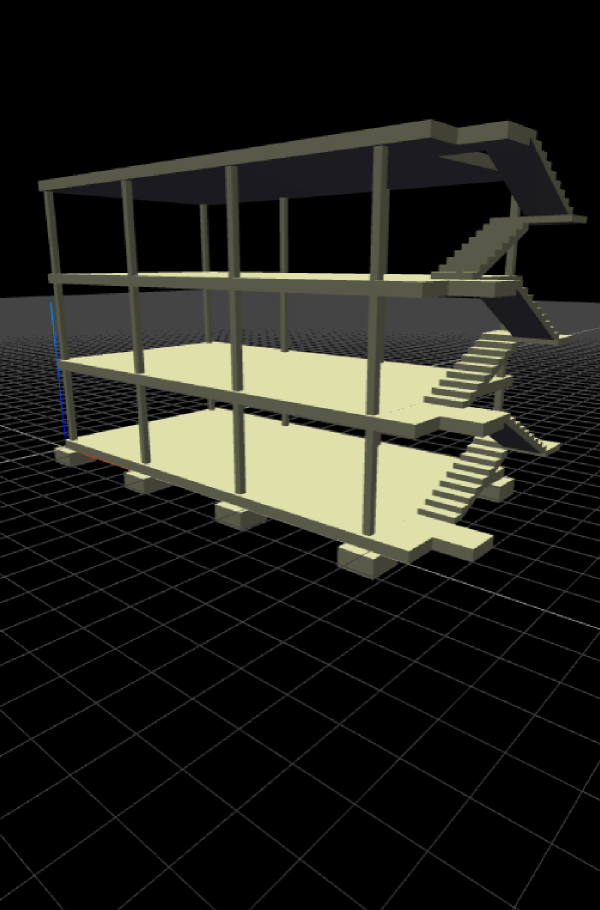
\includegraphics[width=1.0\linewidth]{./images/all_examples/dom_ino_crop}
    \caption{Dom-ino}
    \label{fig:ex:domino}
  \end{subfigure}
  \begin{subfigure}[b]{0.3\linewidth}
    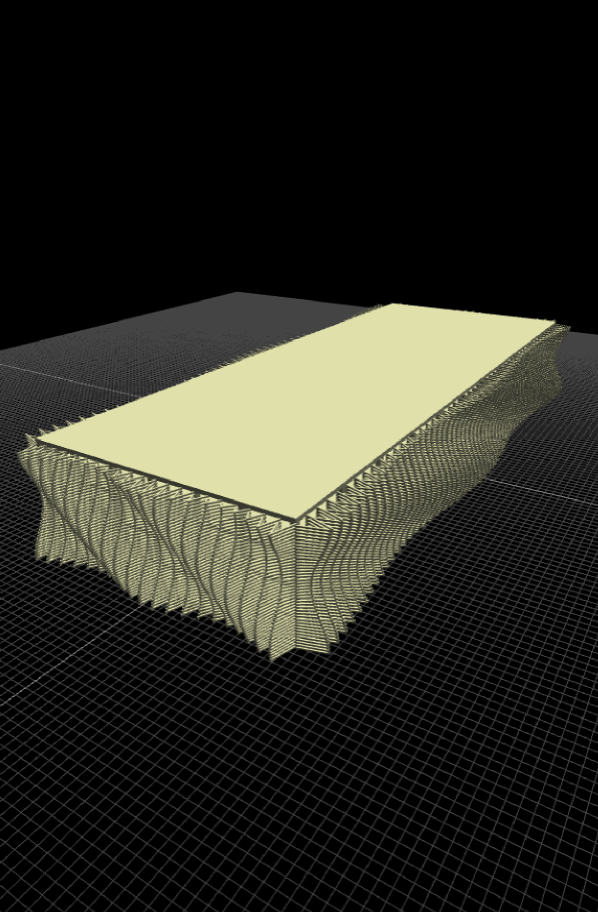
\includegraphics[width=1.0\linewidth]{./images/all_examples/edificio_carmo_crop}
    \caption{Carmo Facade}
    \label{fig:ex:carmo:facade}
  \end{subfigure}
  \begin{subfigure}[b]{0.3\linewidth}
    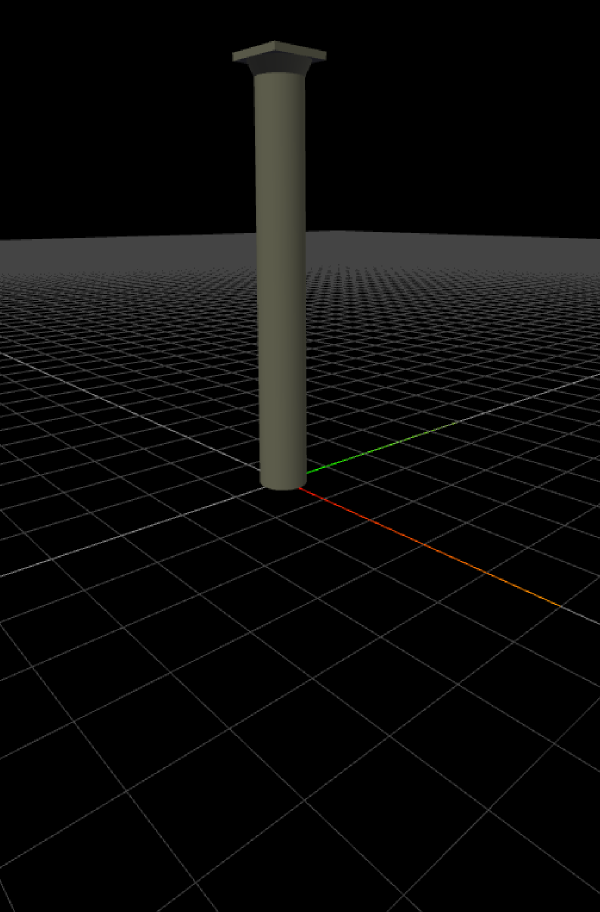
\includegraphics[width=1.0\linewidth]{./images/all_examples/column_crop}
    \caption{Column}
    \label{fig:ex:column}
  \end{subfigure}
  \begin{subfigure}[b]{0.3\linewidth}
    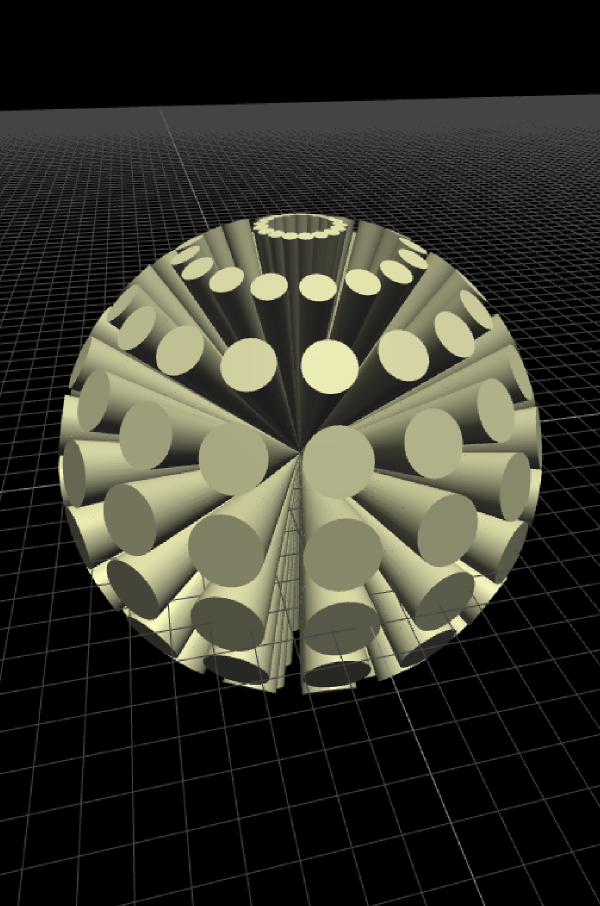
\includegraphics[width=1.0\linewidth]{./images/all_examples/coneSphere_crop}
    \caption{Sphere of cones}
    \label{fig:ex:cone:sphere}
  \end{subfigure}
  \begin{subfigure}[b]{0.3\linewidth}
    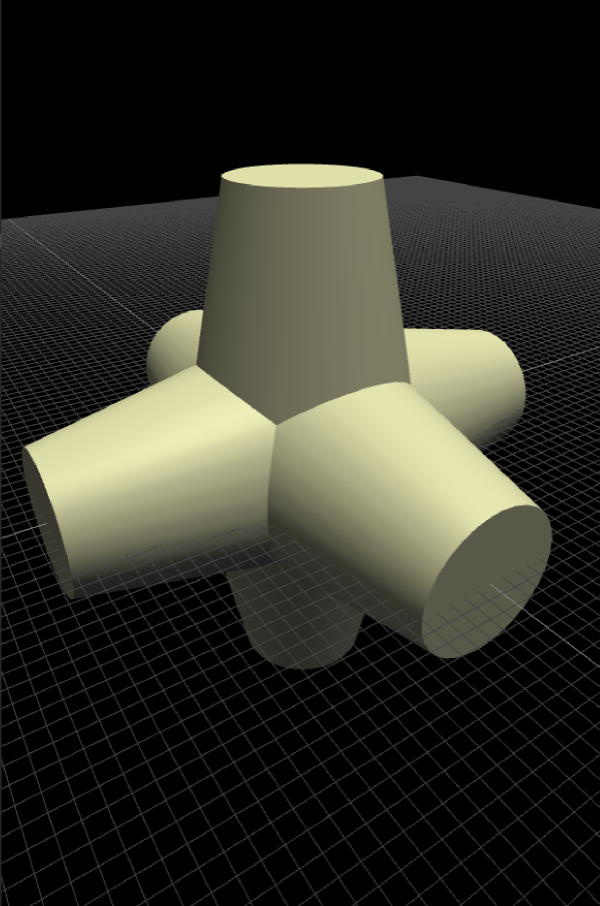
\includegraphics[width=1.0\linewidth]{./images/all_examples/ortho_cones_crop}
    \caption{Orthogonal Cones}
    \label{fig:ex:ortho:cones}
  \end{subfigure}

  %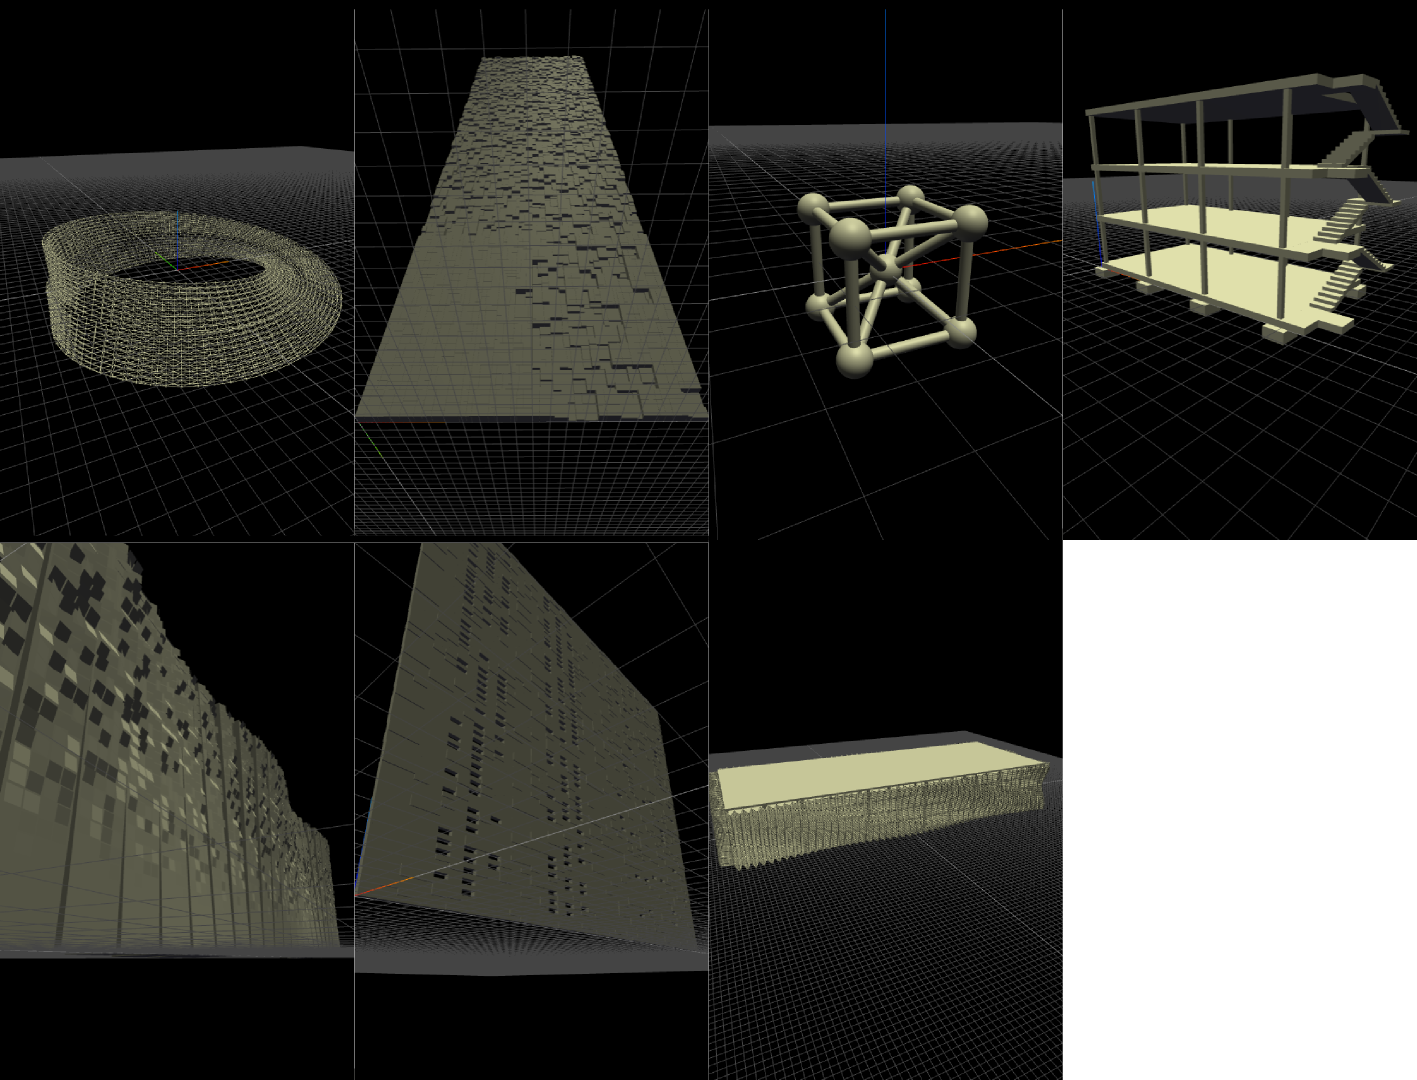
\includegraphics[width=12cm]{./images/all_examples}
  \caption{Renderings of results of the implemented example programs.}
  \label{fig:all:examples}
\end{figure}


%\section{Real Use}
%{\it This is where I give the prototype to an architect, ask him to do a building, get his feedback, and tell it to the world.}


\section{Performance}
\label{sec:eval:performance}
There are several areas where performance plays an important part when using the environment.

To evaluate our solution's performance, we have tested several situations: (1) we compared program running times in the web page with running times of the same programs in Rosetta; (2) we compared program running times with export times; (3) we compared how traceability data collection affects program running times; and (4) we compared export times with times from running programs directly in Rosetta.

\paragraph{Setup}
All tests were performed on a computer with an Intel Core i7-3630QM CPU, 16GB DDR3 RAM and an AMD Radeon HD 7970M GPU.

The web page and the remote CAD service were hosted at the same computer.

%The source code of each program used in the tests can be found in Appendix~\ref{appendix:test:source:code}. %{\bf(either here, appendix or github)}

\begin{figure}
  \centering
  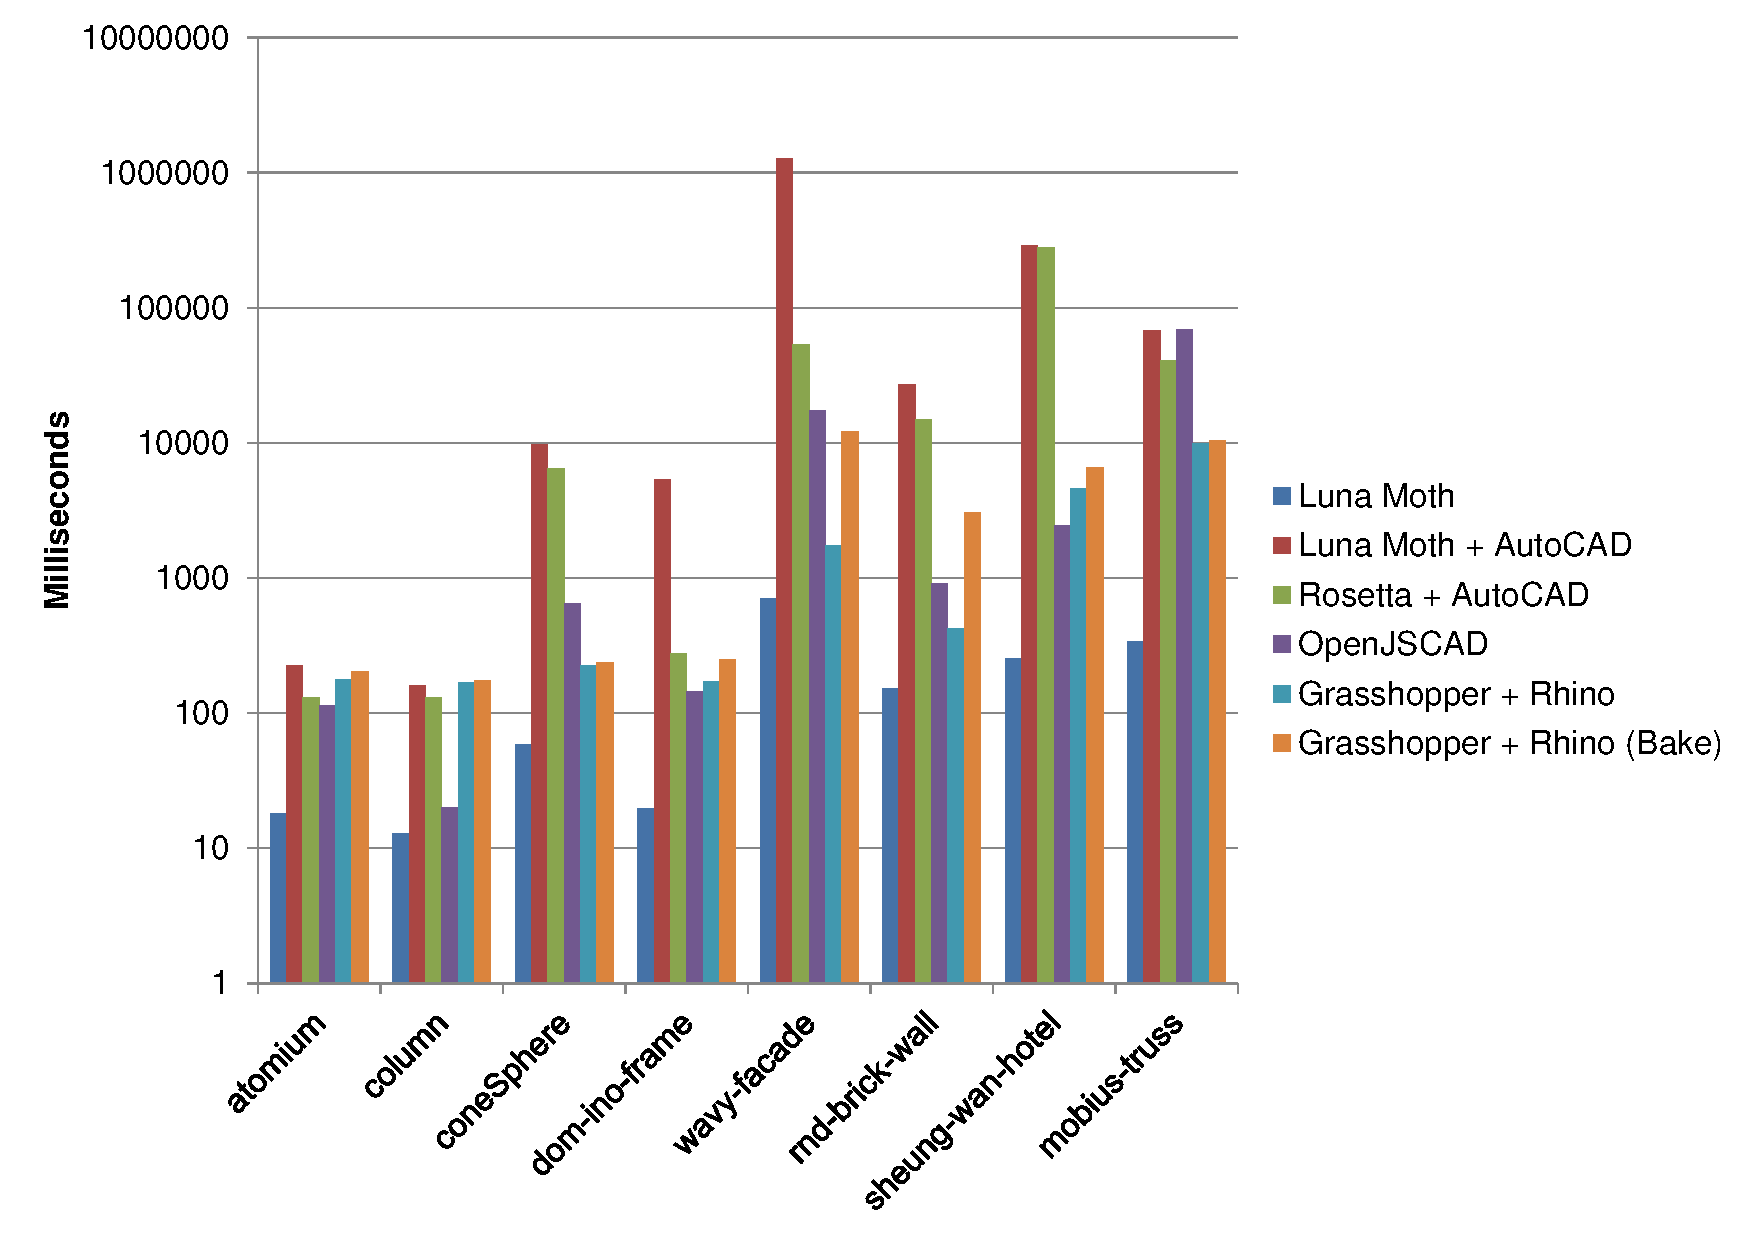
\includegraphics[width=12cm]{./images/run_export_rosetta_times}
  \caption{Comparison of running times for the web, the export process and Rosetta.}
  \label{fig:run:export:rosetta:chart}
\end{figure}



\subsection{Running Performance}
Our solution should provide immediate feedback to architects, therefore letting them easily understand the correlation between the program inputs and outputs\cite{Leitao2014illustrated}.
Apart from making it easy to change program inputs, it needs to run programs and show results as fast as possible.
It is important to compare the performance of our solution to the performance of other systems that can also provide immediate feedback.

To see how the performance of our web-based \gls{gd} environment compares to the existing environments, we compared the time each takes to generate identical models.
First, we implemented a version of the program using each environment's programming language and, then, measured the time each took to complete.
The times can be seen in Figure~\ref{fig:run:export:rosetta:chart}.
Times are the average of three runs.

As can be seen, the relationship between running times varies from program to program, although the web page is consistently faster than Rosetta connected to AutoCAD.
More specifically, Rosetta's running times for both the Mobius and Ines Wall programs are around 40x the running times on the web page.
% and around 500x for the Sheung-Wan Hotel program.

With this in mind, we can say that our solution can provide better feedback than Rosetta.

%We compared our environment with Rosetta (using the OpenGL backend), OpenJSCAD and Rhino+Grasshopper.


\subsection{Export Performance}
When time comes to pass on the building design to other people that use different tools --- like mechanical, electric, plumbing services or even other architects --- the architect must provide it in a format compatible with their tools.
This has been covered in our solution by letting the program that generates the building model run in a \gls{cad} tool.

The next step was to evaluate how the execution time differs between the normal running process and the remote \gls{cad} running process.
To measure the difference, we ran two example programs using both processes and measured the time each took to complete.
The chart in Figure~\ref{fig:run:export:rosetta:chart} shows the running times of two programs for each process.
Times are the average of three runs.

As seen in the chart, comparing export times to normal running times, export times are around 200x the normal running times for Mobius Truss, and 170x the normal running times for Ines Wall.

Given the difference of two orders of magnitude, it is highly preferable to get feedback using the web page instead of using the export process.
The export process should be reserved to actually export to \gls{cad}.

One may need some clarification on how this difference appears.
For each primitive call a program does, data has to be converted, sent over an HTTP connection to the remote CAD service, passed to Rosetta, then to the \gls{cad} application to perform the primitive, and finally the result must be sent back to the web page.
The difference comes from the time needed for \gls{cad} applications to execute operations and from the time spent on communication between applications.
As shown in \cite{Leitao2014illustrated}, \gls{cad} applications are not well suited for \gls{gd} since they were designed to support human interaction and, therefore, are not ready for the amount of operations produced by \gls{gd} programs.


\subsection{Export vs Rosetta}
As shown in Chapter~\ref{chapter:solution}, Rosetta plays an important part in the process used by our environment to send results to \gls{cad} applications.
Rosetta acts as an interface to communicate with \gls{cad} applications, while remote CAD service makes that interface available to the web page as a web service.
Due to the fact that our solution uses Rosetta as an intermediate to export to \glspl{cad}, it is interesting to assess how much time the process adds to running a program that produces the same results using just Rosetta.

To measure the difference, we selected two programs and measured the time each took to export and to run in Rosetta.
The two systems use different programming languages, therefore, each program had two versions, one for our solution and one for Rosetta.
Figure~\ref{fig:run:export:rosetta:chart} shows the running times for each system, grouped by program.

Looking at the graph, we see that export times are $\approx$4.1x the times of running directly in Rosetta for Mobius Truss and that export times are $\approx$4.3x the times of running directly in Rosetta for Ines Wall.

As with the export time evaluation, the increase in running times comes from the overhead in communication between the web page and the remote CAD service.
Moreover, although during export programs are first run in the web page and Rosetta's role is reduced to make them happen in the \gls{cad}, results are still sent one by one to the remote CAD service meaning that a lot of time is spent transmitting data.

Unlike with the export time evaluation, this comparison lets us distinguish the time of transmitting data from the time taken by Rosetta and the \gls{cad} application to apply operations.


\subsection{Traceability Performance}
Collecting traceability data requires that additional work must be done when a program is being executed.
The additional work will inevitably increase the time it takes to finish executing the program.
This can make the environment less capable of giving immediate feedback, therefore having a negative impact in its the usage experience.

To measure the impact that traceability data collection has on program running time, we have selected a small set of programs, ran them with data collection and without it, and measured the time each took to execute.
The chart in Figure~\ref{fig:traceability:timing} shows a comparison of their times, grouped by program.
Times are the average of six runs.

We can observe that running with traceability impacts the running time, increasing it by 20--30\%.
The impact is indeed significant.
Like so, traceability data collection may need to be disabled to increase feedback when running complex programs.
However, the impact is worth taking when the user wants to get a better understanding of the program.

\begin{figure}
  \centering
  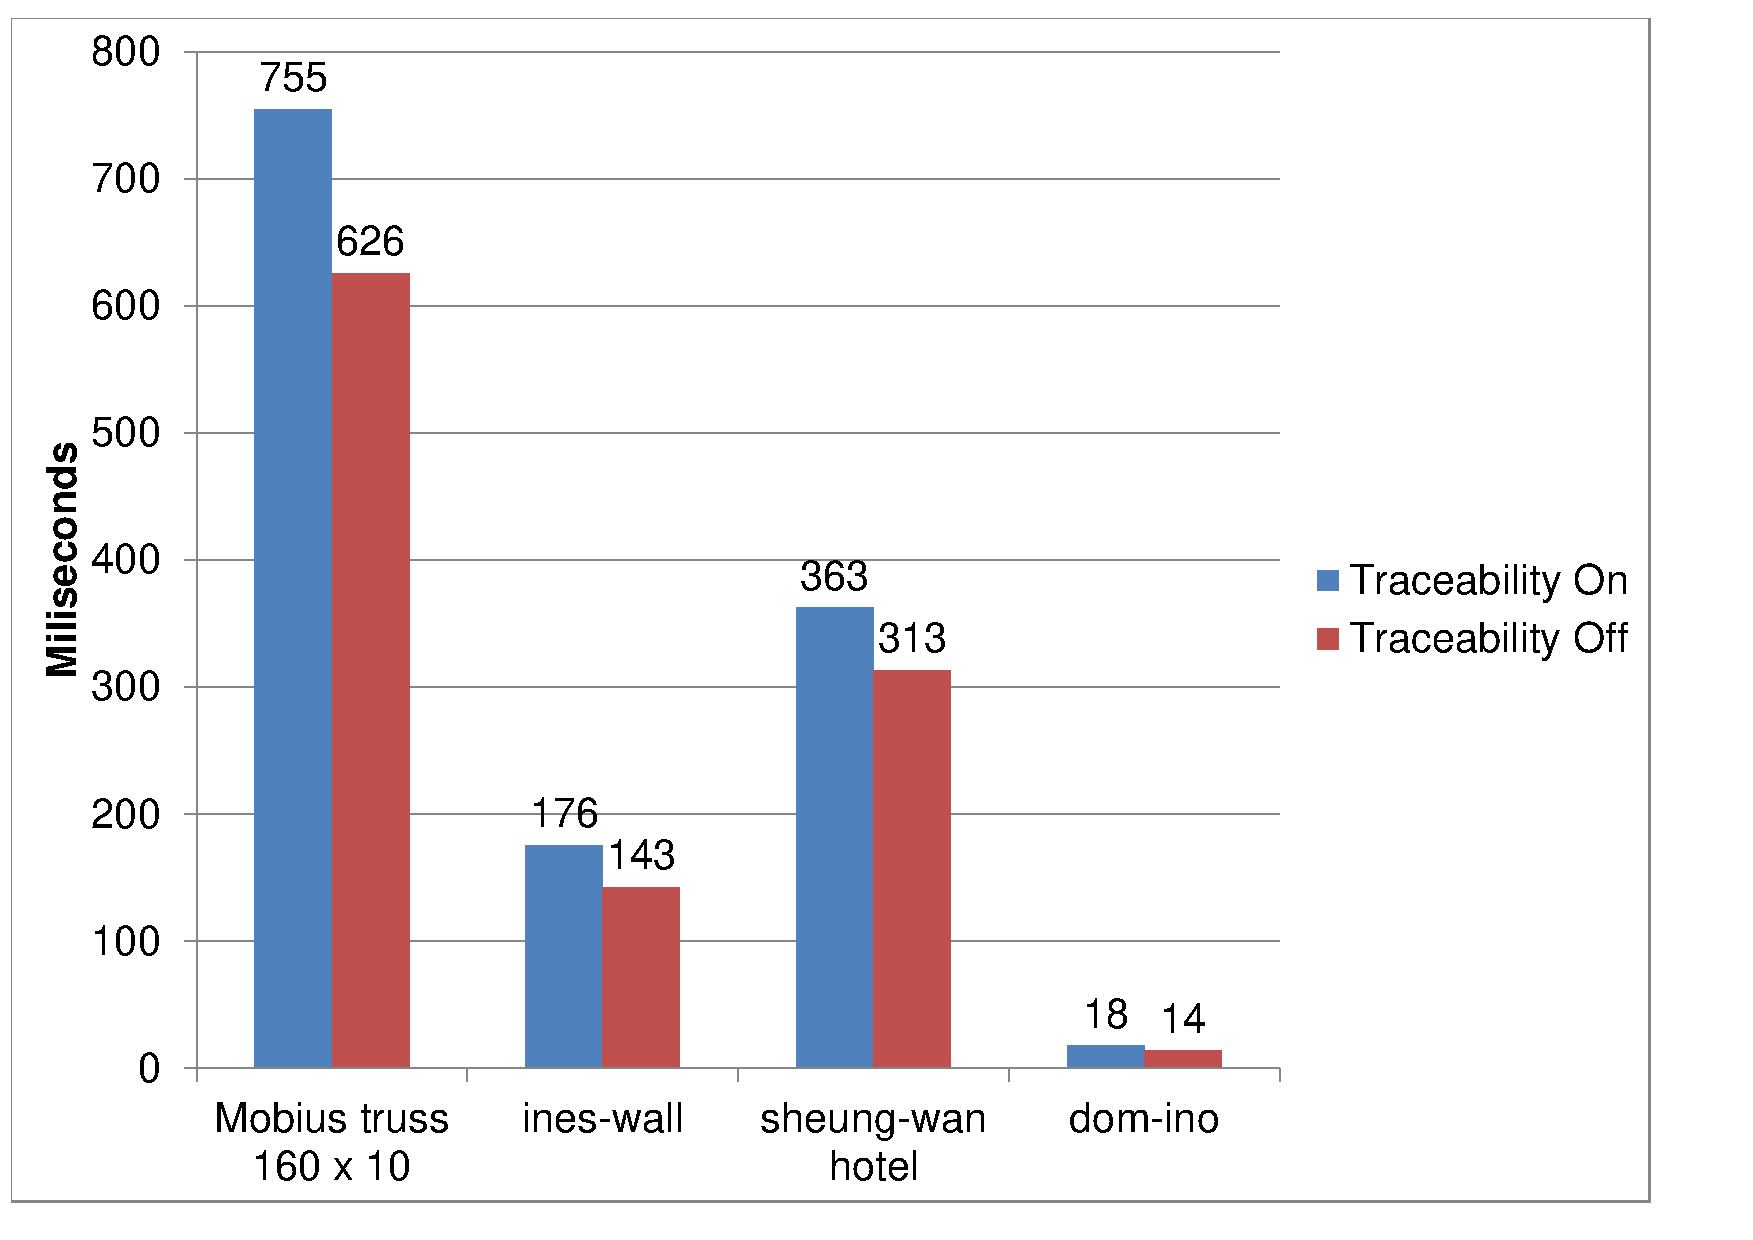
\includegraphics[width=12cm]{./images/traceability_timing}
  \caption{Running while collecting traceability data and while not collecting traceability data.}
  \label{fig:traceability:timing}
\end{figure}




%Describe possible programming techniques using the IDE / our solution.
%- Examples of use (made by me)
%- Example from architect (e.g. Inês Caetano)
%Describe possible use cases using our solution.

%GD capabilities(examples)
%- Architect example
%- More examples
%Performance:
%- web page vs rosetta vs grasshopper/dynamo
%- running in web page vs running in remote CAD service
%- impact of traceability tracking
%Geometry/primitives: our solution vs existing solutions

%Usefulness of traceability?
